\documentclass[11pt,letterpaper]{article}

\usepackage[margin=0.85in]{geometry}
\usepackage{fontspec}
\usepackage{xeCJK}
\setmainfont{Times New Roman}
\setCJKmainfont{Microsoft YaHei}
\usepackage{graphicx}
\usepackage{hyperref}
\usepackage{enumitem}
\usepackage{setspace}
\usepackage{tabularx}
\usepackage{array}

\hypersetup{colorlinks=true, allcolors=black}
\setlist[itemize]{leftmargin=1.2em, itemsep=0.25em, topsep=0.15em, parsep=0.08em}
\setlength{\parindent}{0pt}
\setlength{\parskip}{0.15em}
\pagestyle{empty}
\setstretch{1.15}

\newlength{\cvdatecol}
\setlength{\cvdatecol}{10.5em}

\newcommand{\sectionheader}[1]{%
  \vspace{0.45em}
  {\large\bfseries #1}\\[-0.15em]
  \rule{\textwidth}{0.4pt}\par
  \vspace{0.2em}
}

\newcommand{\cvline}[3][0em]{%
  \par\nobreak
  \noindent\hspace*{#1}%
  \begin{tabularx}{\dimexpr\textwidth-#1\relax}{@{}X@{\hspace{0.75em}}>{\raggedleft\arraybackslash}p{\cvdatecol}@{}}
  #2 & #3 \\
  \end{tabularx}%
}

\newcommand{\courseline}[1]{%
  \par\addvspace{0.22em}%
  \noindent\hspace*{3.2em}#1\par
}

\begin{document}

\noindent
\begin{minipage}[t]{0.78\textwidth}
{\LARGE\bfseries Ke Cheng HSU (Clio) 許可證}\\[0.4em]
\href{mailto:khsu@connect.ust.hk}{khsu@connect.ust.hk} $\cdot$ +852 6840 9753\\[0.12em]
\href{https://cliohsu1997.github.io}{https://cliohsu1997.github.io/}\\[0.45em]
\textbf{BUSINESS ADDRESS}\\[0.1em]
Department of Economics, 5067 Lee Shau Kee Business Building\\
The Hong Kong University of Science and Technology\\
Clear Water Bay, Kowloon, Hong Kong\\[0.35em]
\textbf{RESEARCH FIELDS}\\[0.1em]
Industrial Organization, Digital Economics, Quantitative Marketing
\end{minipage}%
\hfill
\begin{minipage}[t]{0.20\textwidth}
\vspace{0pt}
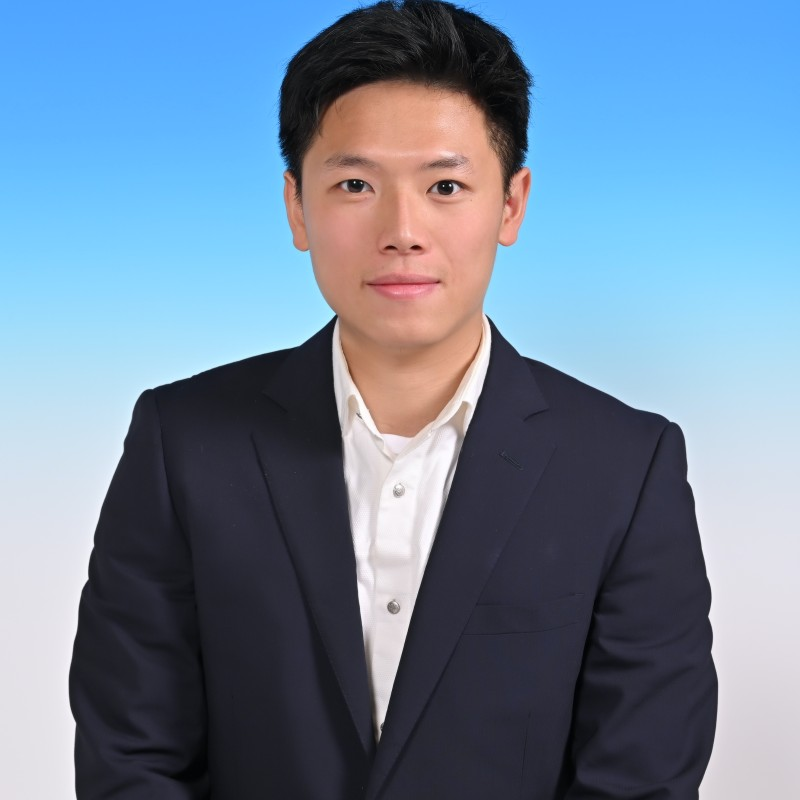
\includegraphics[width=\linewidth]{photo_formal.jpg}
\end{minipage}

\sectionheader{EDUCATION}
{\setstretch{0.88}
Hong Kong University of Science and Technology\\[-0.35em]
\cvline[1.5em]{Ph.D.\ in Economics}{2022 -- 2027 (expected)}
\vspace{-0.15em}
\cvline[1.5em]{M.Phil.\ in Economics}{2020 -- 2022}
\vspace{-0.15em}
\cvline[1.5em]{B.Sc.\ in Mathematics and Economics (Minor in Actuarial Mathematics)}{2015 -- 2019}
}

\vspace{-0.45em}
\sectionheader{WORKING PAPERS}
\begin{itemize}
  \item ``Designing Return Policy in E-Commerce: A Trade-off between Purchase and Return Efficiency'' \textit{(Job Market Paper)}\\[0.15em]
  \textit{Abstract:} We study whether return policies encourage efficient returns and purchases. A stricter policy curbs inefficient ex-post returns, but lower return rates make higher prices more attractive for sellers and can exclude efficient purchases. Using Taobao apparel data, we estimate a structural model of purchase, insurance, and return under monopoly pricing across six categories. Automatic return-shipping coverage performs better in high-margin categories; optional coverage performs better in thinner-margin categories. A menu pairing a discounted price with a medium restocking fee balances both margins for most categories.\\[0.12em]
  \textit{Presented at ($^{\ast}$ scheduled):} APIOC 2026$^{\ast}$; ESAM 2026$^{\ast}$; 中國經濟學年會夏季論壇 2026; HKUST Business School PhD Conference; CEP Brownbag in HKUST.

  \item ``Product Design with Heterogeneous Search Costs'', with Pak Hung AU\\[0.15em]
  \textit{Abstract:} We introduce search-cost heterogeneity into a sequential-search model with differentiated products. In equilibrium, low-search-cost consumers seek niche products and high-search-cost consumers seek standardized products. A fall in search costs can raise prices when the composition effect dominates. Prices also respond asymmetrically to search-cost shocks.\\[0.12em]
  \textit{Presented at:} APIOC 2023; AMES 2023 NTU Singapore.
\end{itemize}

\sectionheader{WORK IN PROGRESS}
\begin{itemize}
  \item ``Too Much Unsold Stock?: Environmental Consequences of Price Commitment'', with Kohei Kawaguchi and Kei Kawai.
  \item ``Pass-Through and Incidence with Product Returns'', with Ce Bian and Liang Zhao.
\end{itemize}

\sectionheader{EXPERIENCE}
{\setstretch{0.88}
\textit{Research}\\[-0.5em]
\cvline[1.5em]{Research Assistant for Prof.\ Benjamin Bernard, National Taiwan University}{2020}

\vspace{-0.1em}
\textit{Teaching}\\[-0.5em]
\cvline[1.5em]{Lecturer, Math Camp for MSc in Economics, HKUST (4.53/5)}{2026}
\vspace{-0.12em}
\cvline[1.5em]{Teaching Assistant Coordinator, Business School, HKUST}{2025 -- 2026}
\vspace{-0.12em}
\cvline[1.5em]{Teaching Assistant, Department of Economics, HKUST (average 4.72/5)}{2020 -- 2025}
\vspace{0.08em}
\courseline{ECON2123 -- Macroeconomics (4.53/5)}
\courseline{ECON4134 / ECON4999T -- Economics of Uncertainty and Information}
\courseline{ECON5210 -- Microeconomic Theory I (4.85/5; 4.82/5)}
}

\sectionheader{FELLOWSHIPS AND AWARDS}
{\setstretch{0.9}
\cvline[1.5em]{Research Travel Grant}{2023; 2026}
\vspace{-0.12em}
\cvline[1.5em]{Red Bird PhD Award}{2022}
\vspace{-0.12em}
\cvline[1.5em]{Postgraduate Studentship from the HKUST}{2020 -- present}
\vspace{-0.12em}
\cvline[1.5em]{Academic Achievement Medal}{2019}
\vspace{-0.12em}
\cvline[1.5em]{University Scholarship (730K HKD)}{2015 -- 2019}
}

\sectionheader{SKILLS}
Technical Skills: R, Python, C++, \LaTeX, AWS\\
Languages: English (fluent), Mandarin (native), Cantonese (basic)

\sectionheader{REFERENCES (THESIS SUPERVISION COMMITTEE)}
{\setstretch{0.92}
\noindent
\begin{minipage}[t]{0.48\textwidth}
\textbf{\href{https://aupakhung.weebly.com/}{Pak Hung AU}}\\
Associate Professor\\
Department of Economics\\
Hong Kong University of Science and Technology\\
\href{mailto:aupakhung@ust.hk}{aupakhung@ust.hk}
\end{minipage}\hfill
\begin{minipage}[t]{0.48\textwidth}
\textbf{\href{https://www.kohei-kawaguchi.com/}{Kohei Kawaguchi}}\\
Associate Professor\\
Department of Economics\\
Hong Kong University of Science and Technology\\
\href{mailto:kkawaguchi@ust.hk}{kkawaguchi@ust.hk}
\end{minipage}

\vspace{1.0em}
\noindent
\begin{minipage}[t]{0.48\textwidth}
\textbf{\href{https://www.e.u-tokyo.ac.jp/fservice/faculty/kawai/kawai-e/kawai01-e.html}{Kei Kawai}}\\
Professor\\
Department of Economics\\
University of Tokyo\\
\href{mailto:kawaixkei@gmail.com}{kawaixkei@gmail.com}
\end{minipage}
}

\end{document}
